\chapter{OSPF: Part 1}\label{ospf-part-1}

\begin{figure}
\centering
\pandocbounded{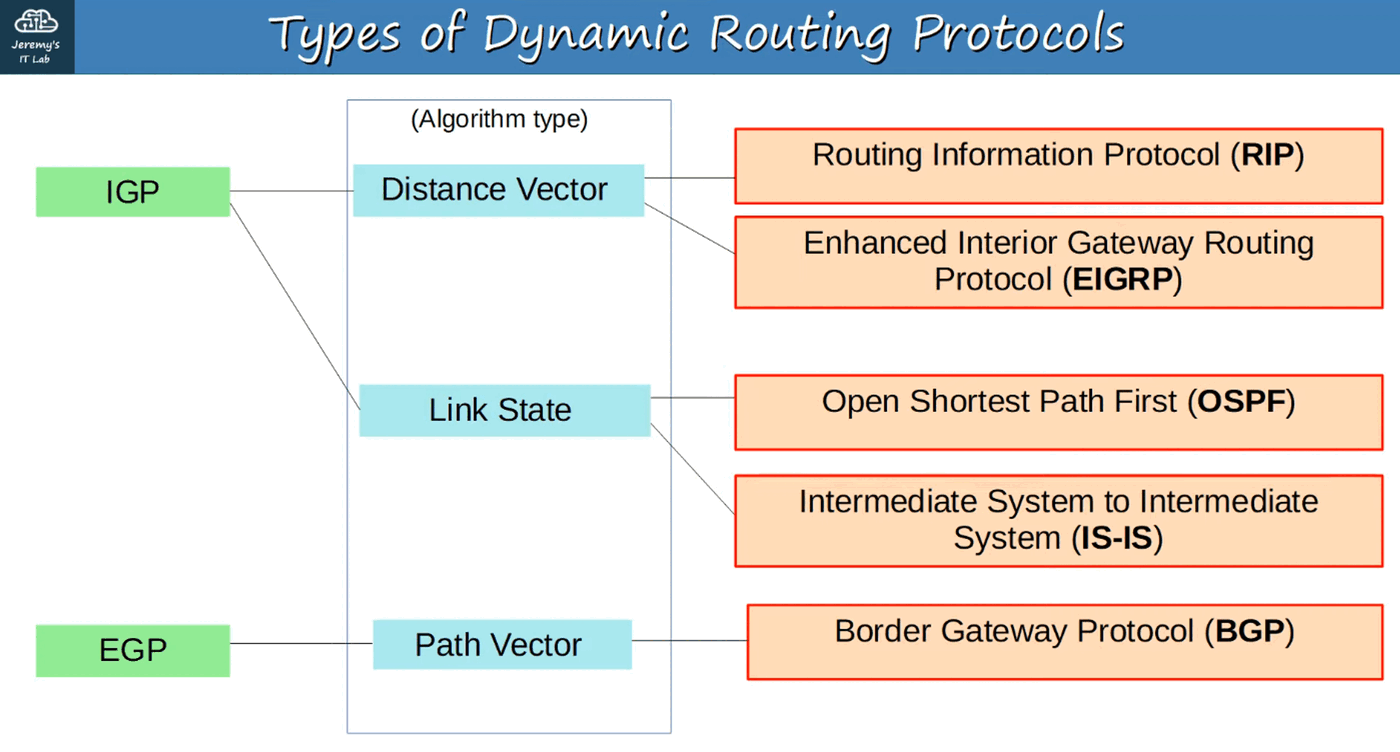
\includegraphics[keepaspectratio,alt={image}]{images/27-ospf-part1/img-001.png}}
\end{figure}

\section{Link State Routing
Protocols}\label{link-state-routing-protocols}

\begin{itemize}
\tightlist
\item
  When using a LINK STATE ROUTING PROTOCOL, every ROUTER creates a
  `connectivity map' of the NETWORK
\item
  To allow this, each ROUTER ADVERTISES information about its INTERFACES
  (connected NETWORKS) to its NEIGHBOURS. These ADVERTISEMENTS are
  passed along to the other ROUTERS, until all ROUTERS in the NETWORK
  develop the same map of the NETWORK
\item
  Each ROUTER independently uses this MAP to calculate the BEST ROUTES
  to each DESTINATION
\item
  LINK STATE PROTOCOLS use more resources (CPU) on the ROUTER, because
  MORE information is shared.
\item
  However, LINK STATE PROTOCOLS tend to be FASTER in reacting to CHANGES
  in the NETWORK than DISTANCES VECTOR PROTOCOLS
\end{itemize}

\section{Basic OSPF Operations}\label{basic-ospf-operations}

\begin{itemize}
\tightlist
\item
  Stands for \textbf{Open Shortest Path First}
\item
  Uses the \textbf{Shortest Path First} algorithm

  \begin{itemize}
  \tightlist
  \item
    Created by Dutch comp. scientist - Edsger Dijkstra
  \item
    aka \textbf{Dijkstra's Algorithm} (Could be Exam Question)
  \end{itemize}
\end{itemize}

THREE Versions:

\begin{itemize}
\item
  OSPFv1 (1989) : OLD, not in use anymore
\item
  OSPFv2 (1998) : Used for IPv4
\item
  OSPFv3 (2008) : Used for IPv6 (can be used for IPv4, but v2 is usually
  used)
\item
  Routers store information about the NETWORK in LSAs (Link State
  Advertisements), which are organized in a structure called the LSDB
  (Link State Database)
\item
  Routers will \textbf{FLOOD} LSAs until all ROUTERS in the OSPF
  \emph{area} develop the same map of the network (LSDB)
\end{itemize}

\begin{figure}
\centering
\pandocbounded{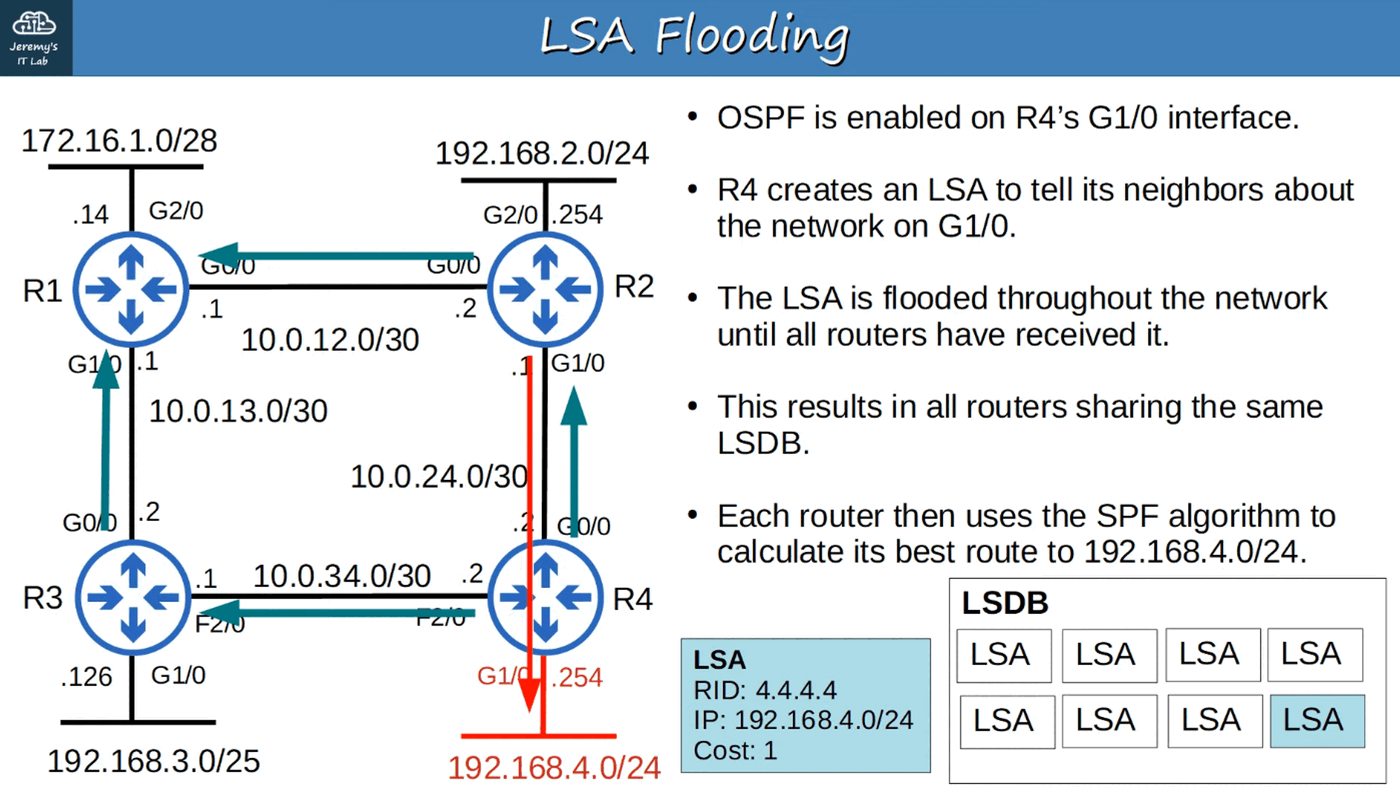
\includegraphics[keepaspectratio,alt={image}]{images/27-ospf-part1/img-002.png}}
\end{figure}

LSA's have an AGING TIMER of 30 Minutes, by Default). The LSA will be
FLOODED again after the timer expires

In OSPF, there are THREE MAIN STEPS in the process of sharing LSAs and
determining the BEST ROUTE to each DESTINATION in the network

\begin{enumerate}
\def\labelenumi{\arabic{enumi})}
\item
  \textbf{BECOME NEIGHBORS} with other ROUTERS connected to same SEGMENT
\item
  \textbf{EXCHANGE LSAs} with neighbor ROUTERS
\item
  \textbf{CALCULATE THE BEST ROUTES} to each DESTINATION, and insert
  them into the ROUTING TABLE
\end{enumerate}

\section{OSPF Areas}\label{ospf-areas}

\begin{itemize}
\tightlist
\item
  OSPF uses \textbf{AREAS} to divide up the NETWORK
\item
  SMALL NETWORKS can be \emph{single-area} without any negative effects
  on performance
\item
  LARGE NETWORKS, \emph{single-area} design can have NEGATIVE effects:

  \begin{itemize}
  \tightlist
  \item
    SPF ALGORITHM takes more time to calculate ROUTES
  \item
    SPF ALGORITHM requires exponentially more processing power on
    ROUTERS
  \item
    Larger LSDB takes up more MEMORY on ROUTERS
  \item
    Small changes in NETWORK cause every ROUTER to FLOOD LSAs and run
    the SPF algorithm again
  \end{itemize}
\item
  By dividing up a large OSPF NETWORK into several SMALLER
  \textbf{\emph{areas}}, you can avoid the above NEGATIVE effects
  (sounds similar to VLANs re: broadcast domains)
\end{itemize}

WHAT IS AN OSPF AREA?

\begin{figure}
\centering
\pandocbounded{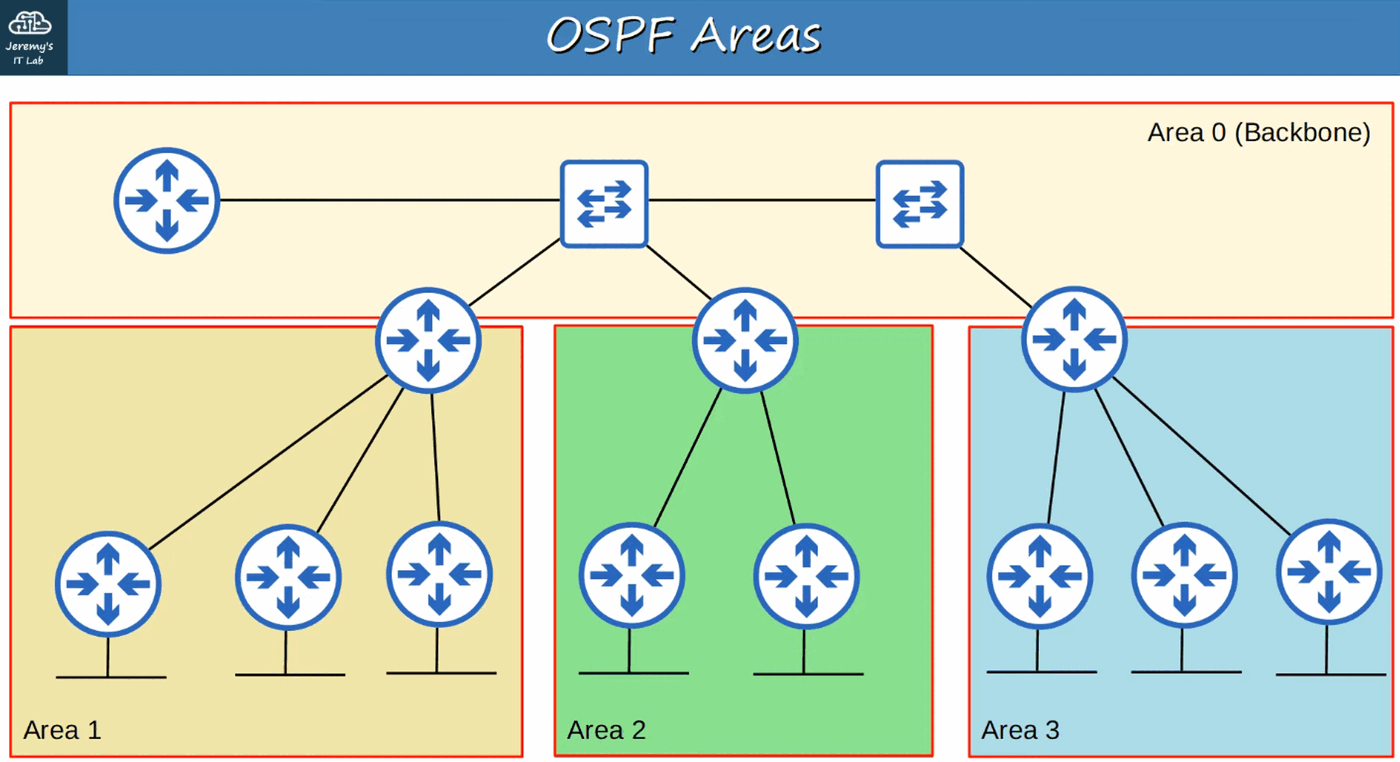
\includegraphics[keepaspectratio,alt={image}]{images/27-ospf-part1/img-003.png}}
\end{figure}

\begin{itemize}
\tightlist
\item
  An \textbf{AREA is} a set of ROUTERS and LINKS that share the same
  LSDB
\item
  The \textbf{BACKBONE AREA} (Area 0) is an AREA that all other AREAS
  must connect to
\item
  ROUTERS with ALL INTERFACES in the SAME AREA are called INTERNAL
  ROUTERS
\item
  ROUTERS with INTERFACES in MULTIPLE AREAS are called \textbf{AREA
  BORDER ROUTERS} (ABRs)
\end{itemize}

ABRs maintain a SEPARATE LSDB for each AREA they are connected to.

It is recommended that you connect an ABR to a MAXIMUM of TWO AREAS.

Connecting an ABR to 3+ AREAS can overburden the ROUTER

\begin{itemize}
\tightlist
\item
  ROUTERS connected to the BACKBONE AREA (Area 0) are called
  \textbf{BACKBONE ROUTERS}
\item
  An \textbf{INTRA-AREA ROUTE} is a ROUTE to a DESTINATION inside the
  same OSPF AREA
\item
  An INTER-AREA ROUTE is a ROUTE to a DESTINATION in a DIFFERENT OSPF
  AREA
\end{itemize}

\section{OSPF Rules}\label{ospf-rules}

\begin{itemize}
\tightlist
\item
  OSPF AREAS should be CONTIGUOUS (no split AREAS)
\item
  All OSPF AREAS must have \emph{at least} ONE ABR connected to the
  BACKBONE AREA
\item
  OSPF INTERFACES in the SAME SUBNET \emph{must} be in the SAME AREA
\end{itemize}

\section{Basic OSPF Configuration}\label{basic-ospf-configuration}

\section{OSPF Area 0}\label{ospf-area-0}

\begin{figure}
\centering
\pandocbounded{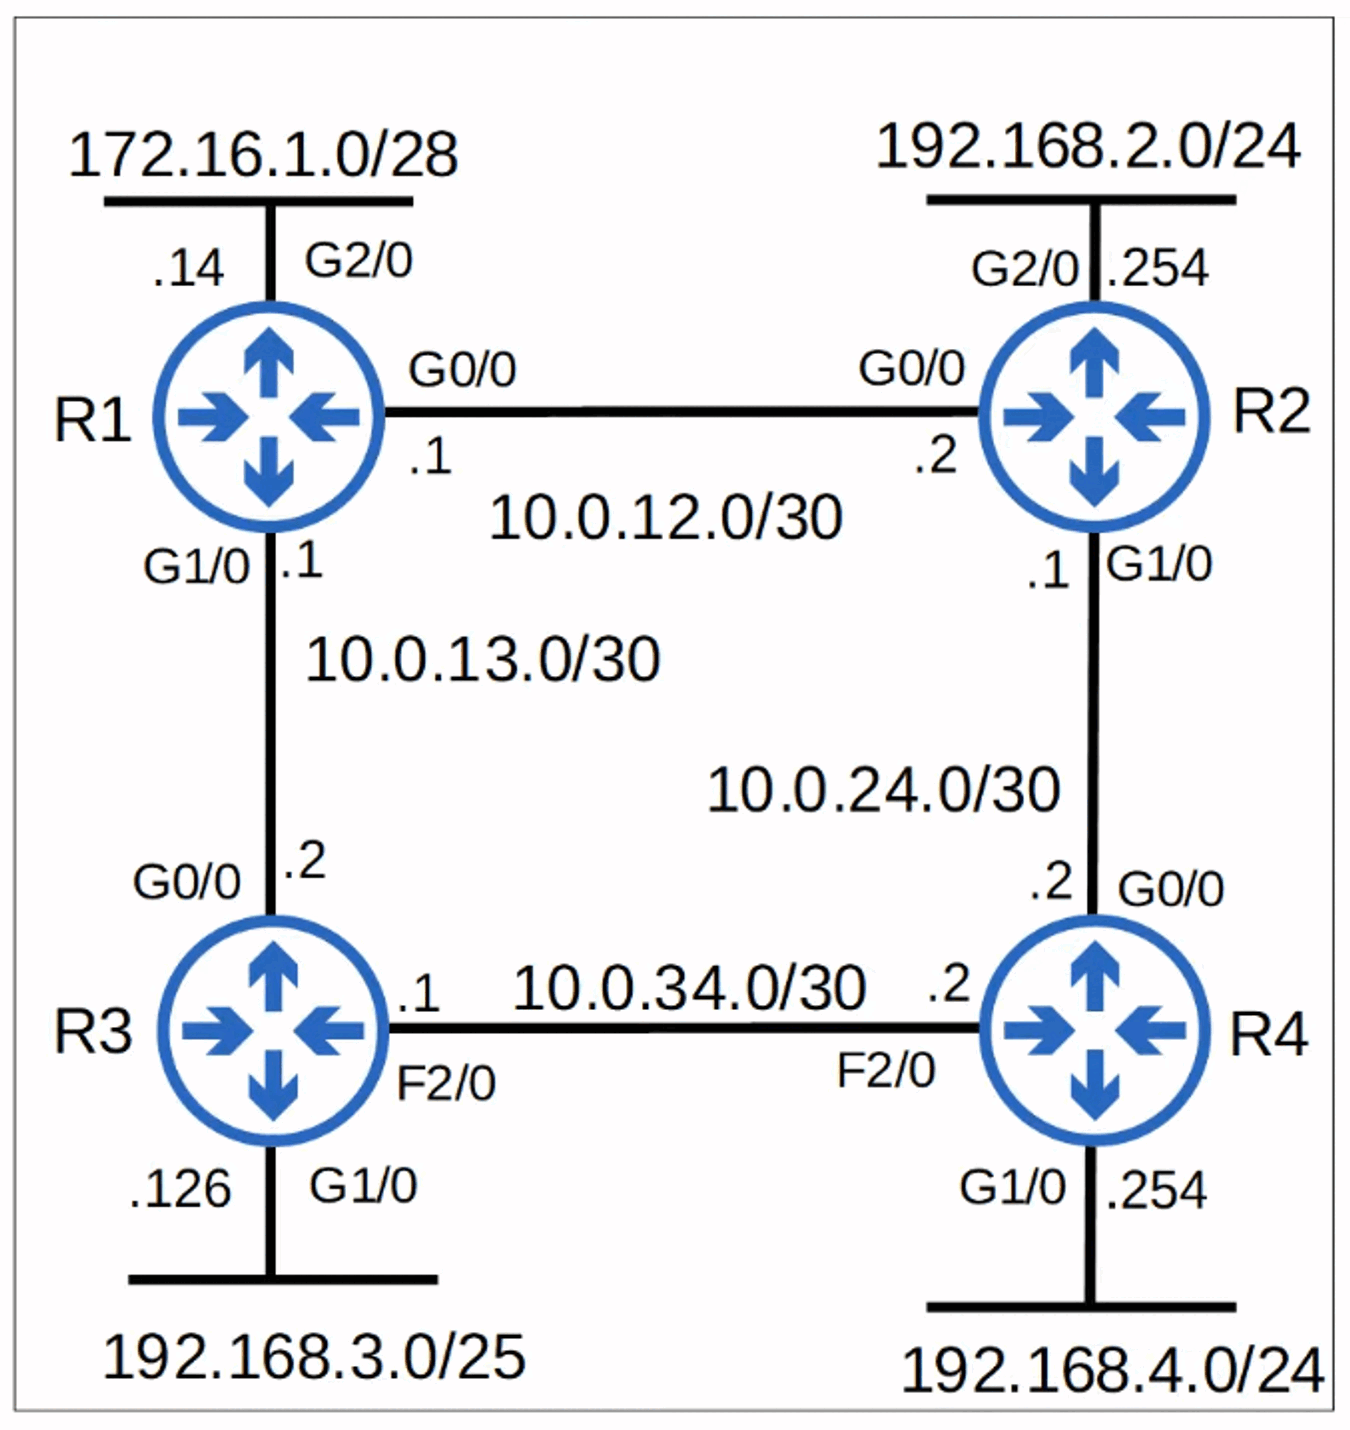
\includegraphics[keepaspectratio,alt={image}]{images/27-ospf-part1/img-004.png}}
\end{figure}

Commands for configuring an OSPF

\begin{figure}
\centering
\pandocbounded{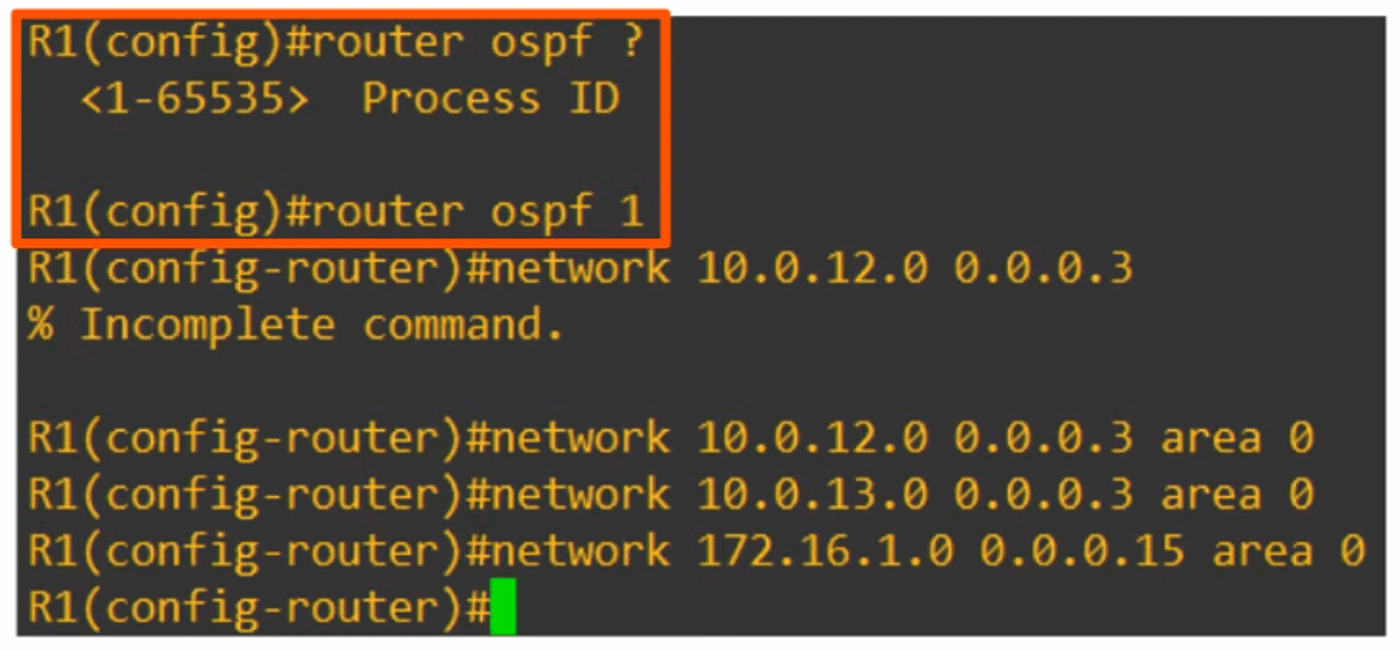
\includegraphics[keepaspectratio,alt={image}]{images/27-ospf-part1/img-005.png}}
\end{figure}

\begin{itemize}
\tightlist
\item
  The OSPF \textbf{Process ID} is \textbf{locally significant.} ROUTERS
  with different Process IDs can become OSPF Neighbors
\item
  The OSPF ``network'' command requires you to specify the AREA (in this
  case, it's ``area 0'')
\item
  For the CCNA, you only need to configure single-area OSPF (AREA 0)
\end{itemize}

The ``network'' command tells OSPF to:

\begin{itemize}
\tightlist
\item
  Look for ANY INTERFACES with an IP ADDRESS contained in the RANGE
  specified in the ``network'' command
\item
  Activate OSPF on the INTERFACE in the specified AREA
\item
  The ROUTER will then try to become OSPF neighbors with other
  OSPF-Activated neighbor ROUTERS
\end{itemize}

\begin{figure}
\centering
\pandocbounded{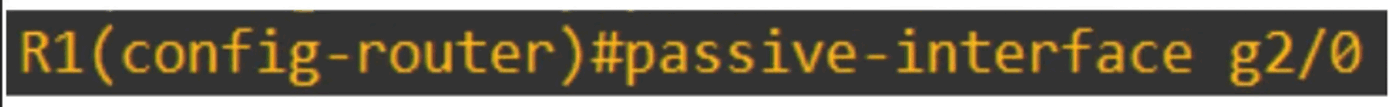
\includegraphics[keepaspectratio,alt={image}]{images/27-ospf-part1/img-006.png}}
\end{figure}

\begin{itemize}
\tightlist
\item
  Know this command from RIP and EIGRP
\item
  The ``passive-interface'' command tells the ROUTERS to stop sending
  OSFP `hello' messages out of the INTERFACE
\item
  However, the ROUTER will continue to send LSA's informing it's
  neighbors about the SUBNET configured on the INTERFACE
\item
  You should ALWAYS USE this command on neighbors which don't have any
  OSPF neighbors
\end{itemize}

\begin{figure}
\centering
\pandocbounded{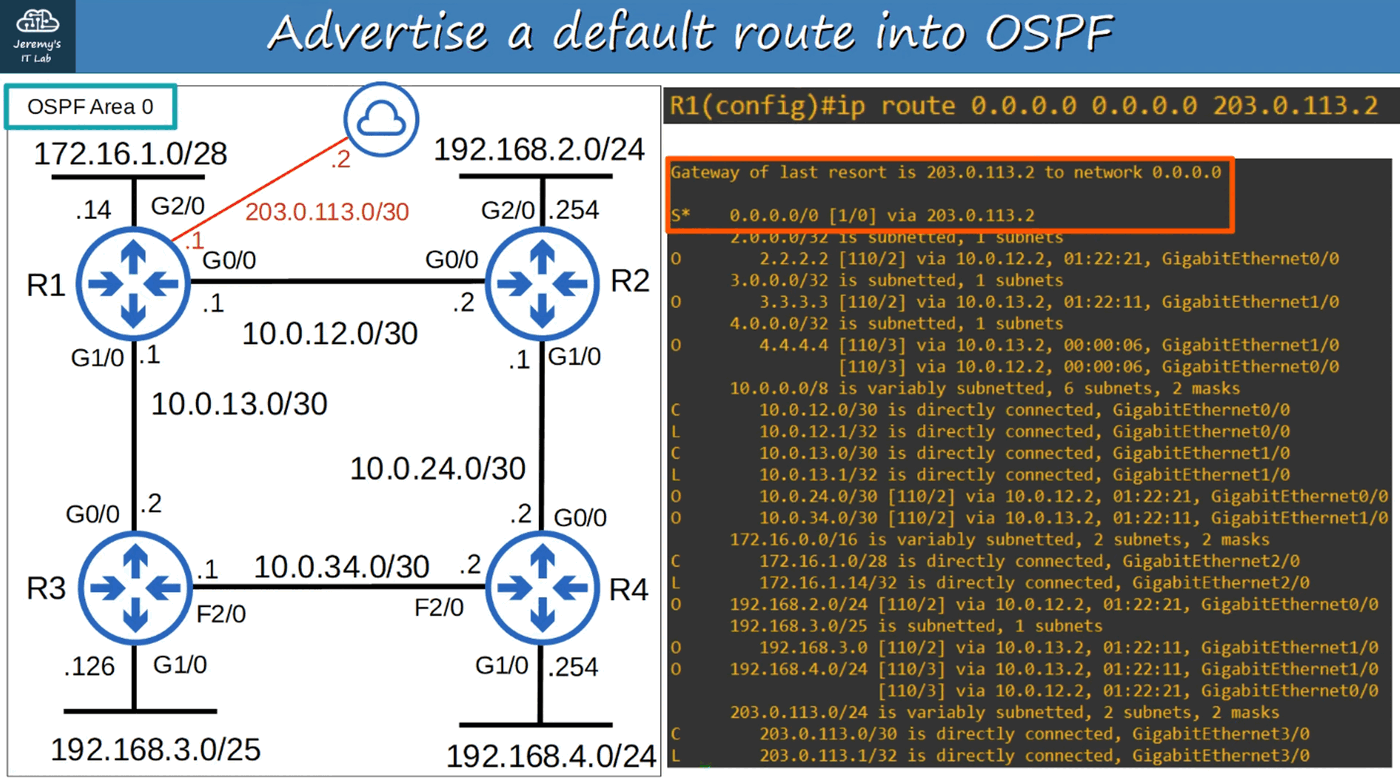
\includegraphics[keepaspectratio,alt={image}]{images/27-ospf-part1/img-007.png}}
\end{figure}

\begin{figure}
\centering
\pandocbounded{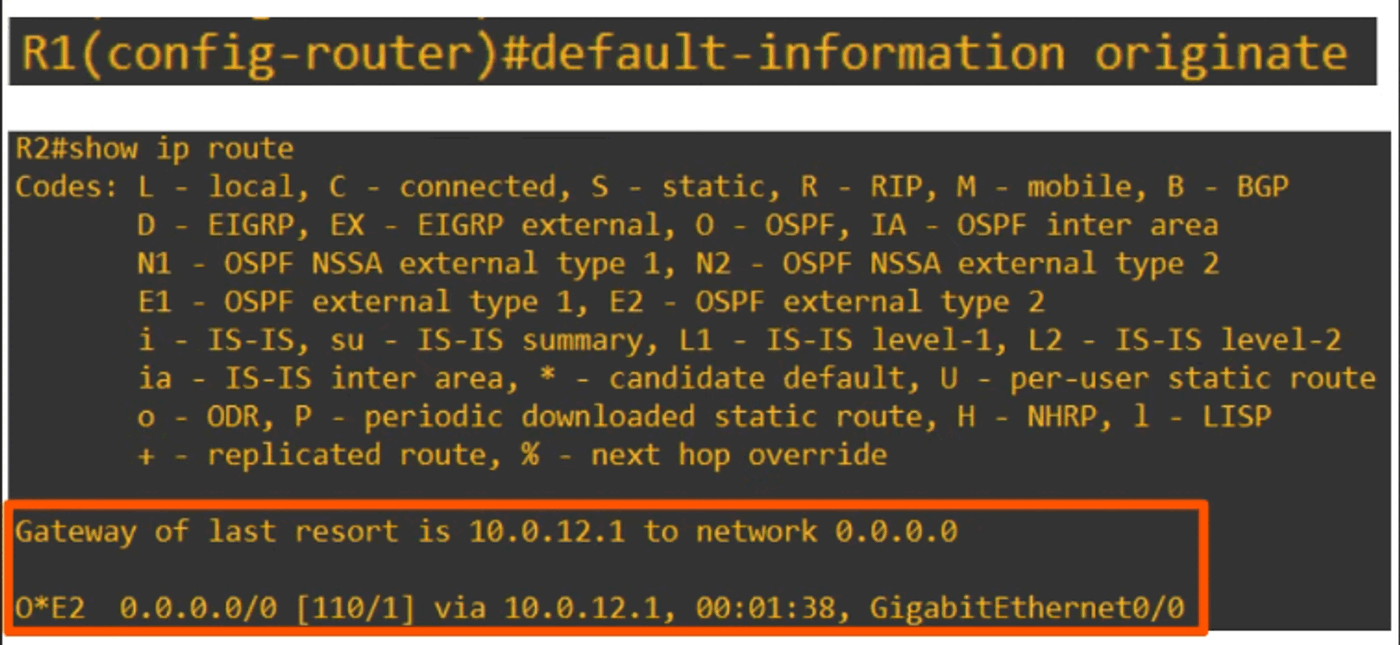
\includegraphics[keepaspectratio,alt={image}]{images/27-ospf-part1/img-008.png}}
\end{figure}

``show ip protocols''

\begin{figure}
\centering
\pandocbounded{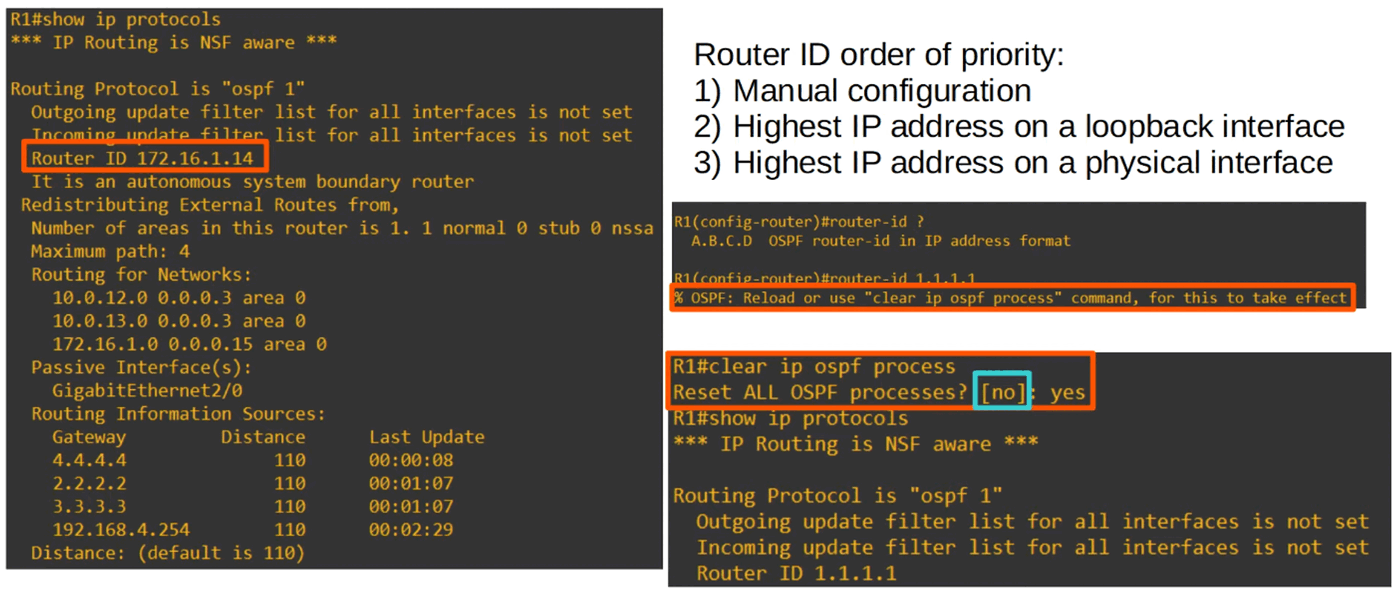
\includegraphics[keepaspectratio,alt={image}]{images/27-ospf-part1/img-009.png}}
\end{figure}

NOTE the ``no'' in square brackets - this indicates this is the DEFAULT
choice

\begin{figure}
\centering
\pandocbounded{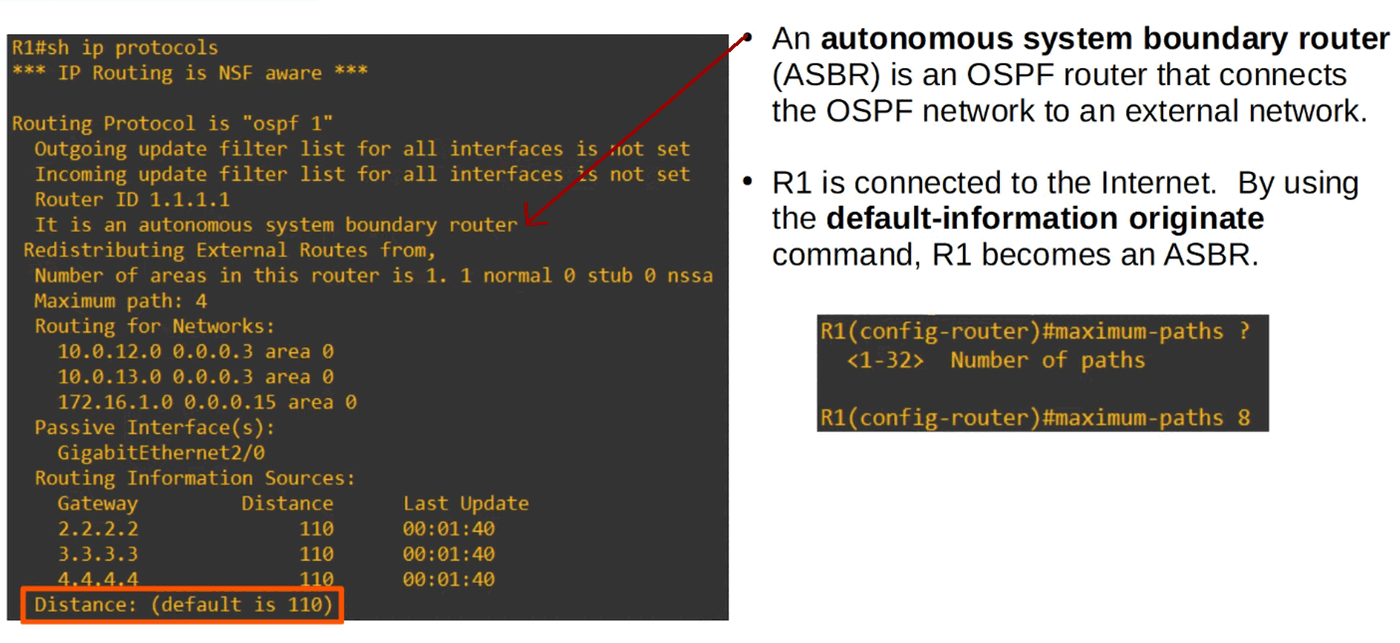
\includegraphics[keepaspectratio,alt={image}]{images/27-ospf-part1/img-010.png}}
\end{figure}

DISTANCE (AD) for OSPF is 110 (DEFAULT) but can be changed with the
``distance'' command

\begin{figure}
\centering
\pandocbounded{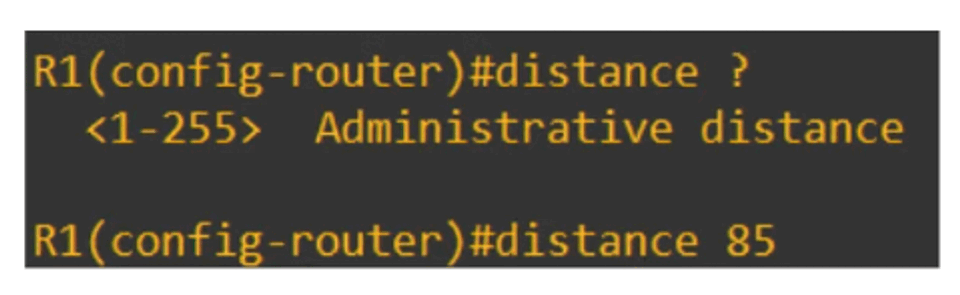
\includegraphics[keepaspectratio,alt={image}]{images/27-ospf-part1/img-011.png}}
\end{figure}
